\documentclass[12pt]{article}
\usepackage{amsmath} % AMS Math Package
\usepackage{amsthm} % Theorem Formatting
\usepackage{amssymb} % Math symbols such as \mathbb
\usepackage[hidelinks]{hyperref}
\usepackage{graphicx}
\usepackage{caption}
\usepackage{filecontents}
\usepackage{subcaption}% Allows for eps images
\usepackage[table,xcdraw]{xcolor}
\usepackage{tikz}
\usepackage{siunitx}
\usepackage{tabularx} % Allows for table with custom column width
\usepackage{lipsum}
\usepackage{parskip}
\usepackage{booktabs}
%\usepackage{mathtools}
\usepackage{geometry} % see geometry.pdf on how to lay out the page. There's lots.
\geometry{a4paper}
\usepackage [english]{babel}
\usepackage [autostyle, english = american]{csquotes}
\usepackage{siunitx}
\usepackage{float}
\usepackage{array}
\usepackage{paralist}
\usepackage{mathtools}
\usepackage{amsmath}
\usepackage{setspace} % you can control the spacing here
\onehalfspacing
\setlength\parindent{24pt}
\MakeOuterQuote{"} % or letter or a5paper or ... etc
\usepackage{cite}% \geometry{landscape} % rotated page geometry
\usepackage{multicol} %allows you to make multiple columed items

%\usepackage[
%natbib=true,
%backend=biber,
%style=ieee,
%citestyle=authoryear,
%maxcitenames=2, 
%uniquelist=false
%]{biblatex}
\usepackage{mathrsfs}
\usepackage{graphicx}
%\addbibresource{sniabib.bib} %Imports bibliography file


\title{}
\author{}
\date{} % delete this line to display the current date

%%% BEGIN DOCUMENT
\begin{document}
\begin{titlepage}
\centering
\Large{\textbf {Your Project Title}}
\vspace{10mm}






\Large\textit{\textbf{T Lucas Makinen}} \\
\vspace{25mm}
\large{Junior Paper \\ Department of Physics \\ Princeton University \\Fall 2018\\}
\begin{figure}[H]
\centering

\includegraphics[scale=0.1]{pton}
\end{figure}
\vspace{1mm}
\normalsize{Advised by:} \\
\normalsize{Professor Roberto Trotta, \textit{Imperial College London}} \\

\normalsize{Professor Lyman A Page, Jr \textit{Princeton University}}\\

\vfill

\vspace*{25mm}
\normalsize{This paper represents my work in accordance with University regulations.}
\begin{center} 
\normalsize{/s/ Your Name}
\end{center}

\end{titlepage}



\newpage
\pagenumbering{roman}
\vspace*{\fill}
\section*{Abstract}

Basically, put spoilers here. You're gunna do great! This document turned out WAY longer than I ever intended it to be, but as I was writing it, I pretty much figured I'd throw up everything I know about LaTeX into a document. I really hope this helps. 

\noindent 

\vspace*{\fill}

\newpage

\tableofcontents

\newpage
\pagenumbering{arabic}



\section{Introduction}

\subsection{Curvature and the Friedmann Equation}

Conclusion: $\lambda$CDM standard model

\section{Measuring Spacetime: Distances in Cosmology}
In the previous section, we introduced the Friedmann equation, which gives us a way to explore possible ways a given universe evolves. To test these models and find values that suit our universe, we need to relate the unitless theoretical quantities $\mathscr{C} = \{\Omega_m, \Omega_{\lamda}$ or $w, h\}$ to a measurable quantity, like distance. With the universe as vast as it is, the sharpest tool we have are the fastest things we can detect: photons.

\subsection{Luminosity Distance}
Thanks to classical physics, we have a way of relating the flux, $f$, or intensity of a light source to its distance and \textit{intrinsic} luminosity, $L$.

Consider a photon source $S$ at a co-moving distance $r_o$ away. Then the flux from that source is given as
\begin{equation} \label{eq:flux}
f = \frac{L}{4\pi d_{L}^2}
\end{equation}

Where $d_L$ is the luminosity distance to the source. 

Armed with the Friedmann equation (derive above?), we have a way to relate luminosity distance $d_L$ to the underlying cosmological parameters, $\mathscr{C}$.
\begin{equation}\label{d_l}
    d_L(z,z,\Omega_m, \Omega_{\Lamda}, w) = \frac{c(1+z)}{\sqrt{|\Omega_k|}}S_k \Big( \int_{0}^{z'} dz[\Omega_m(1+z)^3 + \Omega_{de}(z) + \Omega_k(1+z)^2]^{-1/2} \Big)
\end{equation}
Where the Dark Energy density parameter $\Omega_{de}$ is defined as

\begin{equation} \label{omegade}
\Omega_{de} = \Omega_{\Lambda}\exp \Big[3 \int_{0}^{z'} \frac{1+w(z)}{1+z}dz \Big]
\end{equation}

\section{SNIa in Cosmology}



If the intrinsic

Start with Friedmann equation?


-Define equations of state, curvature and fractions

-move on to SNe as "standardizeable candles"-- can be corrected for magnitude, color, and "stretch" (duration) variability via SALT2


\section{Bayesian Statistics and Inference}
There are two interpretations of probability theory. The most commonly taught form is the \textit{frequentist} method, which links a high number of experimental trials with the probability of an outcome. ~\cite{bayesianmethods}

The other school of thought is the \textit{Bayesian} method. This way of understanding probability is linked to the experimenter's \textbf{\textit{own knowledge}} about an event. As Bayesians, assessing the outcome of an experiment is not dependent on the repeatability of the event, but instead on how much we know about the event before it's even happened. [EDIT]

As a result, Bayesian statistics can help us answer questions about uncertain events that we can't repeat in a lab, like whether or not Greenland permafrost will have melted by 2100. In this situation, frequentist statistics doesn't shed much light on the answer--but, with a Bayesian mindset we can express some idea of how quickly the desert is growing, and even update our understanding with fresh evidence (from satellite data, for example). \cite{bishop_2006}

\subsection{Bayes' Theorem}
Published after his death in 1764, Thomas Bayes' theorem has enjoyed a fair bit of criticism until much recently. The theorem can be directly derived from the two rules of probability:

%\begin{align}


\begin{centering}
\textbf{Probability Rules}

\begin{tabular}{cc}


\textbf{Sum Rule} &     \begin{equation}\label{sumrule}
p(A) + p(\bar{A}) = 1
    
\end{equation}   \\
\textbf{Product Rule} &      \begin{equation}\label{prodrule}
     p(A,B) = p(A | B)p(A)
\end{equation}  \\


\end{tabular}
\end{centering}

Equation \ref{sumrule} simply states that the sum of $p(A)$, the probability of an event A, and $p(\bar{A})$, the probability of \textit{not} A occurring is unity \cite{bayesianmethods}. Equation \ref{prodrule} expresses the probability of A \textit{and} B occuring as the probability of A \textit{given} B times the \textit{marginal probability}, $p(A)$.

Using the symmetry property $p(A,B) = p(B,A)$, we can form the equality
\begin{equation}
    p(B|A)p(A) = p(A | B)p(B) 
\end{equation}
and, rearranging, obtain
\begin{equation}\label{bayes}
    p(B|A) = \frac{p(A | B)p(B)}{p(A)}
\end{equation}

Using the sum rule we can write the denominator $p(A)$ in terms of the numerator:
\begin{equation}
    p(A) = 1 - p(\bar{A}) = \sum_{B}^{} p(A | B)p(B)
\end{equation}
where the rightmost term is just a sum over all events B, not A. \cite{bishop_2006} The power in this approach to probability becomes much more powerful if we put it into terms of observed and unobserved data.

Consider a vector of observed, "hatted" data, $\hat{\mathscr{D}}$, and a set of unknown parameters, $\theta$, whose values you wish to know about. Subbing these values into Bayes' theorem, we obtain
\begin{equation}\label{databayes}
    p(\theta|\hat{\mathscr{D}}) = \frac{p(\hat{\mathscr{D}} | \theta)p(\theta)}{p(\hat{\mathscr{D}})}
\end{equation}

Equation \ref{databayes} is an expression for $p(\theta |\hat{\mathscr{D}} )$ the \textit{posterior} distributions of $\theta$ given observed $\hat{\mathscr{D}}$. The first term in the numerator, $p(\hat{\mathscr{D}} | \theta)$ is known as the \textit{likelihood}. This is the distribution that describes how likely it is to obtain the observed data given the parameters we're after. Frequentists seek to maximize this quantity by increasing the number of observed data. \cite{bayesianmethods} To the right, $p(\theta)$ is the \textit{prior}, describing how we think the unknown parameters are distributed \textit{before we observe any data $\hat{\mathscr{D}}$}.

Finally, the denominator is the marginalized data probability, which normalizes our posterior distribution. In a lot of cases, this term is ignored, and we can simply write
\begin{equation}
       p(\theta|\hat{\mathscr{D}}) \propto p(\hat{\mathscr{D}} | \theta)p(\theta)
\end{equation}


\subsection{Machine Learning background?}
- Introduce supervised vs unsupervised learning

\subsection{Training Inference Methods through Controlled Simulations}
Quick paragraph about how we use detailed simulations to test our inference before we unleash it on real data.

\subsection{SNIa Selection Effects}
When observing SNIa in the distant universe, intrinsically brighter supernovae are intuitively easier to see. More specifically, we can say that intrinsically brighter SNe at higher redshifts (z>1) tend to have a higher probability of being observed. Once observed, brighter SNe (lower B-band magnitude $m_B$) tend to have a better signal-to-noise (STN) ratio to be followed up for spectroscopic analysis ~\cite{shariff_2017}. Selection probability has also been shown to depend on finer SN light curve features, namely color, $c$, and duration or 'stretch', $x_1$ ~\cite{chotard_etal, guy_etal}. 

SHOW MODULUS BY REDSHIFT PLOT


\section{Selection Function}


- logistic regression overview: how $1/1+e^x$ maps real line between 0 and 1.
- serves as a \textit{classifier}
- supervised learning problem: train and test data


The standard bias correction procedure is to manually adjust observed distance moduli at higher redshifts. [EXPAND UPON AND EXPLAIN FREQUENTIST FART]

By contrast, BAHAMAS seeks to correct this bias in a forward manner. Instead of back-correcting the data once it's observed, we wish to incorporate a bias correction conditional on the \textit{theoretical latent values} of $m_B, c,$ and  $x_1$. We do this by introducing a \textit{selection function} to the inference procedure. This function assigns a probability of selection to each SN$_i$ based on its [OBSERVED] value of parameters $\phi_i = \{m_B, c, x_1\}$.

We're interested in stretching a function between two distinct classes, $\mathscr{C_{k}}$. This is called a \textit{two-class} classification problem. [SHOW PROOF?] ~\cite{bishop_2006}


To simplify notation, we're going to assign a variable $Z$ to each SN. $Z = \{1 =$ `selected',  $0 =$ `missed' \}




To do this, we need a continuous function of each data vector, $\phi_i$ that maps each continuous parameter between 0 and 1. The \textit{logistic sigmoid function} does exactly this: 
\begin{equation}\label{sigmoid}
  p_i = \frac{1}{(1 + e^{-f(\phi_i)})} 
\end{equation}

Where 
\begin{equation}\label{fofphi}
    f(\phi_i) = \beta_{m_B}m_{Bi} + \beta_{c}c_i + \beta_{x_1}x_{1i} + \epsilon 
\end{equation}

We're interested in fitting the coefficients $\beta_j$ 


-BAHAMAS will take into account selection effects at high redshift, as well as dust color correction at low redshift.



\begin{figure}[h!]
\centering
   %\lowcaption
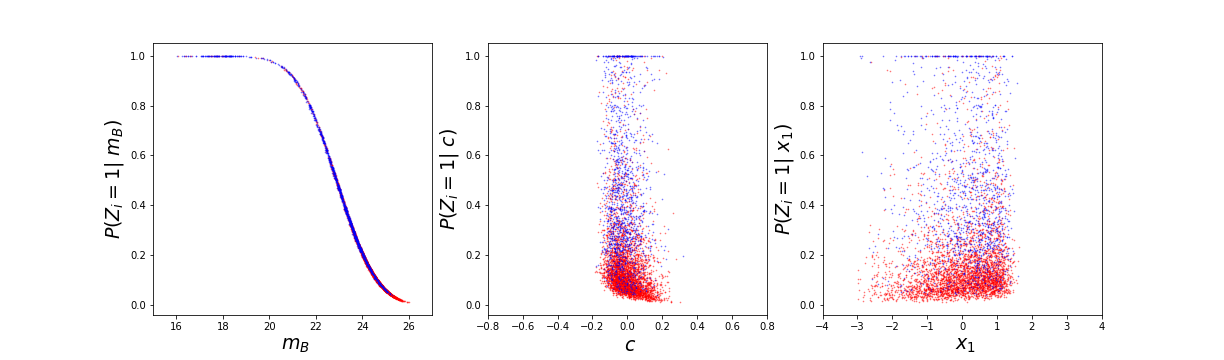
\includegraphics[width=\textwidth]{selection_fn.png}
\caption{The selection function shown with respect to each latent variable; apparent B-band magnitude $m_B$ (left), color $c$ (middle), and stretch $x_1$ (right). We train our logistic model using 25\% of the simulated dataset, and proceed to test it on the remaining 75\%. Shown here are the test SNIa. The color scheme shows the truth values of selection. Blue points represent SNe that were truly "selected" in the simulation, while red represents "missed" SNe.}
\label{selectionfn}
\end{figure}


\section{Conclusion}

Working with LaTeX can be messy and honestly I don't understand all of it either. Sometimes you really have to fiddle around with formatting stuff until it finally does what you want it to do. I haven't covered everything and you'll definitely have to do a lot of Google-ing along the way, but I hope you find at least some of the things I've listed here helpful. Always reach out to me with any questions at all! Best of luck, I know you're going to knock your JP out of the park. 



\clearpage
\addcontentsline{toc}{section}{References/Acknowledgements}
\bibliographystyle{h-physrev}
\bibliography{sniabib.bib}

\newpage
\section*{Acknowledgements}

Always a good idea to acknowledge who helped you out here! For me, I got this format from Professor Tully, and he helped me figure out how a lot of LaTeX works. He's great!
 




\end{document}
